%% \begin{figure}[t]
%%   \hrulefill
%%   \begin{center}
%%   \begin{tabular}{cc}%@{\hskip 20pt}c}
%%     \begin{tikzpicture}
%%       \node (p) {$p$};
%%       \node[right=+40pt of p] (p') {$p'$};

%%       \path[->]
%%       (p) edge [bend left] node[above] {$a$}  (p')
%%       (p') edge [bend left] node[above] {$\co{a}$}  (p);
%%     \end{tikzpicture}
%%     &
%%     \begin{tabular}{l@{\hskip 4pt}c@{\hskip 0pt}l}
%%       \begin{tikzcd}
%%       p \arrow[r, "\co{\aa}"]
%%       &
%%       p' \arrow[d, "\aa"]
%%       \\
%%       &
%%       q
%%     \end{tikzcd}
%%     &$\Rightarrow$&\,\,
%%     $p \st{ \tau } q$ or $p = q$
%%     %% \begin{tikzcd}
%%     %%   p
%%     %%   \arrow[r, "\co{\aa}"]
%%     %%   \arrow[d, "\alpha"]
%%     %%   &
%%     %%   p' \arrow[d, "\alpha"]
%%     %%   \\
%%     %%   p'' \arrow[r, "\co{\aa}"]
%%     %%   &
%%     %%   q
%%     %% \end{tikzcd}
%%     \end{tabular}
%%     \\[5pt]
%%     \boom
%%   %%   \begin{tabular}{c}
%%   %%   \begin{tikzcd}
%%   %%     p \arrow[r, "\aa"]
%%   %%     &
%%   %%     p' \arrow[d, "\co{\aa}"]
%%   %%     \\
%%   %%     &
%%   %%     \equiv p
%%   %%   \end{tikzcd}
%%   %% \end{tabular}
%% &

%%     \fwdfeedback
%%   \end{tabular}
%%   \end{center}
%%   \caption{Axioms of forwarders.}
%%   \label{fig:axioms-forwarders}
%%     \hrulefill
%% \end{figure}


%% there is a macro?
\section{Preorders based on \AcceptanceSets}

\label{sec:bhv-preorder}

We first recall the definition of the standard alternative preorder~$\asleq$,
and show how to use it to characterise~$\testleqS$ in our asynchronous setting.
%
We also present a new characterisation that disregards the order of non-causally
related actions.
%
We then explain the tools we use to prove these characterisations, and in
particular their soundness.
%
This section ends with the coinductive version~$\coindleq$ of~$\asleq$,
which we use to prove the hoisting refinement~\eqref{eq:mailbox-hoisting}.

%% In this section we recall the definitions of the %two
%% standard alternative preorders~$\asleq$ and~$\msleq$.
%% Then we show how to use~$\asleq$ to characterise~$\testleqS$ in our setting%. We then use this result to
%% , and then rely on this result to
%% prove that also~$\msleq$ captures the \mustpreorder.

%We achieve the first result by showing that, merely by lifting LTSs of
%output-buffered agents with feedback to LTSs of forwarders,~$\asleq$ captures~$\testleqS$.

% for any LTS of output-buffered agents with feedback.
%In fact we show how to adapt the alternative preorder~$\asleq$ was introduced by \cite{DBLP:books/daglib/0066919}
%To characterise~$\testleqS$ %in~\CCS, and then
%we show that,


%% In the synchronous setting a standard fashion to capture the must preorder
%% is to compare how related processes converge along traces, and how their
%% potential deadlocks match. We clarify this last point.

\subsection{Trace-based characterisations} 
%{\bfseries The acceptance-set approach.} % 
The {\em ready set} of a program~$\server$ is defined as
\coqLTS{ready_set} $R( \server ) = I( \server ) \cup O( \server )$,
and it contains all the {\em visible} actions that~$\server$ can
immediately
% (i.e. strongly)
perform.  If a program~$\server$ is
stable, \ie it cannot perform any
% further step of computation ($\tau$-transition),
$\tau$-transition, we say that it is a {\em potential
  deadlock}.  In general, the ready set of a potential
deadlock~$\server$ shows how to make~$\server$ move to a different
state, possibly one that can perform further computation: if
$R( \server ) = \emptyset$ then there is no way to make~$\server$ move
on, while if~$R( \server )$ contains some action, then~$\server$ is
% essentially
a state waiting for the environment to interact with it.
Indeed, potential deadlocks are called {\em waiting states}
in~\cite{DBLP:conf/ecoop/HondaT91}.
In particular, in an asynchronous setting the outputs of a
% potentially deadlocked program~$\server$
potential deadlock~$\server$ show how~it %$\server$
can unlock the inputs
of a client, which in turn may lead the client to a novel state that
can make~$\server$ move, possibly to a state that can perform further
computation.
%This further motivates the intuition of a {\em potential} deadlock.
A standard manner to capture all the ways out of the potential
deadlocks that a program~$\server$ encounters after executing a
trace~$\trace$ is its {\em acceptance set}:
$\accP{ \server }{ \trace }{ \st{} } = \setof{ R( \stateA ) }{ \state \wt{ \trace } \stateA \stable }$.

In our presentation we indicate explicitly the third parameter of
$\mathcal{A}$, \ie the transition relation of the LTS at hand, because
when necessary we will manipulate this parameter.
For any two LTSs $\genlts_\StatesA, \genlts_\StatesB$ and servers
  $ \serverA \in \StatesA, \serverB \in \StatesB$, we 
  write $\accP{ \serverA }{ \trace }{\st{}_\StatesA} \ll \accP{
    \serverB }{ \trace }{ \st{}_\StatesB}$ %whenever
  if for every $R \in \accP{
    \serverB }{ \trace }{ \st{}_\StatesB}$
% $R \in \acc{ \serverB }{ \trace }$
there exists $\widehat{R} \in \accP{ \serverA }{ \trace }{\st{}_\StatesA}$
% $\widehat{R} \in \acc{ \serverA }{ \trace}$
such that $\widehat{R}
  \subseteq R$.
  We can now recall the definition of the behavioural preorder à la
  Hennessy, $\asleq$, which is based on acceptance
  sets~\cite{DBLP:books/daglib/0066919}.

  \newcommand{\cnvalongLTS}[2]{ \Downarrow_{#1} #2 }

   \begin{definition}\coqMT{bhv_pre}
  \label{def:accset-leq}%
  \label{def:standard-char}
%%   For every $\genlts_A, \genlts_B$, and servers $\serverA \in A, \serverB \in B$ we let
%%   $$
%%   \begin{array}{lcll}
%%     \serverA \bhvleqone \serverB & \text{whenever} & \forall \trace \in \Actfin \suchthat
%%     \serverA \cnvalongLTS{\StatesA}{ \trace } \implies \serverB \cnvalongLTS{\StatesB}{ \trace }
%%     \\[5pt]
%%     \serverA \bhvleqtwo \serverB  & \text{whenever} & \forall \trace \in \Actfin \suchthat
%%       \serverA \cnvalongLTS{\StatesA}{ \trace }  \implies \\
%%       && %\multicolumn{2}{l}{
%%         \accP{ \serverA }{ \trace }{ \st{}_{\StatesA} }
%%       \ll \accP{ \serverB }{ \trace }{ \st{}_{\StatesB} %}
%%     }
%%     \\[5pt]
%% \serverA \asleq \serverB & \text{whenever} & \serverA \bhvleqone
%% \serverB  \text{ and }  \serverA \bhvleqtwo \serverB & \blacksquare
%% \end{array}
  %%   $$
  {We write}
  \begin{itemize}
  \item
    $
    \serverA \bhvleqone \serverB$ whenever $\forall \trace \in \Actfin \suchthat
    \serverA \cnvalongLTS{\StatesA}{ \trace } \implies \serverB \cnvalongLTS{\StatesB}{ \trace }
    $,
    
  \item
    $
    \serverA \bhvleqtwo \serverB$ whenever $\forall \trace \in \Actfin \suchthat
    \serverA \cnvalongLTS{\StatesA}{ \trace }  \implies 
    \accP{ \serverA }{ \trace }{ \st{}_{\StatesA} }
    \ll \accP{ \serverB }{ \trace }{ \st{}_{\StatesB} }
    $,
  \item
    $\serverA \asleq \serverB$ whenever $\serverA \bhvleqone
    \serverB  \text{ and }  \serverA \bhvleqtwo \serverB$.\hfill$\blacksquare$
  \end{itemize}  
   \end{definition}

In the synchronous setting, the behavioural preorder~$\asleq$ is closely related to the denotational semantics
based on Acceptance Trees  proposed by Hennessy in
\cite{DBLP:journals/jacm/Hennessy85,DBLP:books/daglib/0066919}.
There the predicates need not be annotated with the LTS that they are used on,
because those works treat a unique LTS.
Castellani and Hennessy~\cite{DBLP:conf/fsttcs/CastellaniH98} show in their Example~4 that
the condition on acceptance sets, \ie $\bhvleqtwo$, is too demanding
in an asynchronous setting.
  %%%%%%%%%%%%%%%%%%%%%%%%%%%%%% OLD DEFINITION %%%%%%%%%%%%%%%%%%%%%%%%%%%%%%%%%%%%%%%%%%%%%%%
%%   \begin{definition}\coqMT{bhv_pre}
%%   \label{def:accset-leq}%
%%   \label{def:standard-char}
%%   For every $\genlts_A, \genlts_B$, and servers $\serverA \in A$
%%   and $\serverB \in B$ we let
%%   $$
%%   \begin{array}{lcll}
%%     \serverA \bhvleqone \serverB & \text{whenever} & \forall \trace \in \Actfin \suchthat
%%     \serverA \cnvalong{ \trace } \implies \serverB \cnvalong{ \trace }
%%     \\[5pt]
%%     \serverA \bhvleqtwo \serverB  & \text{whenever} \\
%%     & \multicolumn{2}{l}{\forall \trace \in \Actfin \suchthat
%%       \serverA \cnvalong{ \trace }  \implies \acc{ \serverA }{ \trace }
%%       \ll \acc{ \serverB }{ \trace }
%%     }
%%     \\[5pt]
%% \serverA \asleq \serverB & \text{whenever} & \serverA \bhvleqone
%% \serverB  \text{ and }  \serverA \bhvleqtwo \serverB & \blacksquare
%% \end{array}
%%   $$
%% \end{definition}
  %%%%%%%%%%%%%%%%%%%%%%%%%%%%%% OLD DEFINITION%%%%%%%%%%%%%%%%%%%%%%%%%%%%%%%%%%%%%%%%%%%%%%%

   %%% CORRECT AND IMPLEMENTED
%% \ilacom{In page 4 we wrote:\\
%%   ``To reason simultaneously on different LTSs, we will use the
%%   symbols~$\genlts_A$ and~$\genlts_B$ to denote respectively some
%%   LTS~$\lts{\StatesA}{L}{\st{}_A}$ and some
%%   LTS~$\lts{\StatesB}{L}{\st{}_B}$.'' \\
%%   So, if we want to define the preorder $\bhvleqtwo$ between two
%%   servers $\serverA \in A$ and $\serverB \in B$, we should use
%%   $\accP{ \server }{ \trace }{ \st{}_A }$ and
%%   $\accP{ q }{ \trace }{ \st{}_B }$ in the definition above. To be
%%   completely rigorous we should also add indices $A$ and $B$ to the
%%   respective convergence predicates, namely write
%%   $\server \cnvalong_A{\trace }$ and $q \cnvalong_B{\trace }$.}
%In particular in~\cite{DBLP:books/daglib/0066919}, Hennessy does not need to annotate the

%% \ilacom{In fact,
%%   in~\cite{DBLP:conf/fsttcs/CastellaniH98} we said that acceptance
%%   sets were too generous ;-)...  Indeed, acceptance sets are too
%%   generous in the sense that they include also inputs, while inputs
%%   should not be observable in an asynchronous setting.  It is the
%%   preorder $\bhvleqtwo$ that becomes too demanding when using such
%%   acceptance sets.} to capture the \mustpreorder in the asynchronous
%% setting.
%
%, \ie ${\testleqS} \not\subseteq {\asleq}$.
%% The argument is that while the equality $\Nil \testeqS \aa.\co{\aa}$ is
%% true, we have $\aa.\co{\aa} \bhvleqtwo \Nil$, and thus to
%% $\aa.\co{\aa} \asleq \Nil$.
%%\ilacom{??? Something wrong here. Besides, this is not Example~4.}
Letting $\serverA = \aa.\Nil$ and $\serverB = \Nil$, they show that
$\serverA \testleqS \serverB $ but $ \serverA \not \asleq \serverB$,
because $\acc{ \serverA }{ \epsilon } =\set{\set{a}}$ and
$\acc{ \serverB }{ \epsilon } =\set{\emptyset}$, and corresponding to
the ready set $\emptyset \in \acc{ \serverB }{ \epsilon }$ there is no
ready set $\widehat{R} \in \acc{ \serverA }{ \trace}$ such that
$\widehat{R} \subseteq \emptyset$. %
%
%%% NEW EXPLANATION THAT FOLLOWS ILARIA SUGGESTIONS
%
Intuitively this is the case because acceptance sets treat inputs and
outputs similarly, while in an asynchronous setting only outputs can
be tested.

%In the next subsection we present
%\ila{We next present} a technique that
%lets us nevertheless use~$\asleq$ to characterise~$\testleqS$.
Nevertheless~$\asleq$ characterises~$\testleqS$, if servers
are enhanced as with forwarding. We now introduce this concept.

%% We now \gb{present a} technique that is sufficient
%% for~$\asleq$ to characterise~$\testleqS$.


%% OLD EXPLANATION
%% Intuitively this is true because acceptance sets (1) treat inputs and
%% outputs similarly, while \ila{in an asynchronous setting} only outputs
%% can be tested; and (2) they disregard the role of interactions due to
%% spurious messages in the global mailbox.  \ilacom{The second point is
%%   cryptic. Moreover there has been no mention of the global mailbox so
%%   far.} We now define and discuss a technique that is sufficient to
%% for~$\asleq$ to characterise~$\testleqS$.


\paragraph{Forwarders}
We say that an LTS~$\genlts$ is of output-buffered agents {\em with forwarding},
for short is \obaFW, if it satisfies all the axioms in
\rfig{axioms} except \outputfeedback, and also the two following axioms:% in \rfig{axioms-forwarders}.

\begin{equation}
  \label{eq:axioms-forwarders}
  \begin{tabular}{cc}%@{\hskip 20pt}c}
    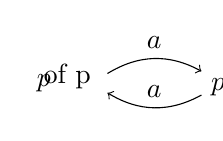
\begin{tikzpicture}
      \node (p) {$p$};
      \node[right=+40pt of p] (p') {$p'$};

      \path[->]
      (p) edge [bend left] node[above] {$a$}  (p')
      (p') edge [bend left] node[above] {$\co{a}$}  (p);
    \end{tikzpicture}
    &
    \begin{tabular}{l@{\hskip 4pt}c@{\hskip 0pt}l}
      \begin{tikzcd}
      p \arrow[r, "\co{\aa}"]
      &
      p' \arrow[d, "\aa"]
      \\
      &
      q
    \end{tikzcd}
    &$\Rightarrow$&\,\,
    $p \st{ \tau } q$ or $p = q$

    \end{tabular}
    \\[5pt]
    \boom
&

    \fwdfeedback
  \end{tabular}
  \end{equation}

The~\boom axiom states a kind of input-enabledness property,
which is however more specific as it
stipulates that the target
state of the input should loop back to the source state via a
complementary output. This is the essence of the behaviour of a
forwarder, whose role is simply to pass on a message and then get
back to its original state.
The~\fwdfeedback axiom is a weak form of Selinger's~\outputfeedback
axiom, which is better understood in conjunction with the~\boom
axiom: if the sequence of transitions $p\st{\out{a}} p'\st{a}q$ in
the~\fwdfeedback axiom is taken to be the sequence of transitions
$p'\st{\out{a}} p\st{a}p'$ in the~\boom axiom, then we see that it
must be $q=p$ in the~\fwdfeedback axiom.  Moreover, no~$\tau$ action is issued when moving from $p$ to $q$, since no
synchronisation occurs in this case: the message is just passed on.

%quiqui
We mechanise all this via the typeclass
\mintinline{coq}{LtsObaFW}. The overall structure of our typeclasses to reason on LTSs is thus
  $\text{\mintinline{coq}{Lts}} \geq \text{\mintinline{coq}{LtsEq}}\geq \text{\mintinline{coq}{LtsOba}}$ and
  $\text{\mintinline{coq}{LtsOba}}$ is a super-class of both \mintinline{coq}{LtsObaFB} and \mintinline{coq}{LtsObaFW}.
%% \begin{center}
%%   \scalebox{.9}{%
%%     \begin{tikzpicture}
%%       \node (Lts) {\lstinline!Lts!};
%%       \node (LtsEq) [right =+7pt of Lts]  {\lstinline!LtsEq!};
%%       \node (LtsOba) [right =+7pt of LtsEq]  {\lstinline!LtsOba!};
%%       \node (LtsFb) [above right=+7pt and +1pt of LtsOba]  {\lstinline!LtsObaFb!};
%%       \node (LtsFw) [below right=+7pt and +1pt of LtsOba]  {\lstinline!LtsObaFw!};
%%       \path[->]
%%       (Lts) edge (LtsEq)
%%       (LtsEq) edge (LtsOba)
%%       (LtsOba) edge (LtsFb)
%%       (LtsOba) edge (LtsFw);
%%     \end{tikzpicture}
%%   }
%% \end{center}
%which %
%we show in \rfig{structure-typeclasses-lts},
%along with the overall structure of our typeclasses to reason on LTSs.
We defer the details to \rapp{coq}.


To prove that~$\asleq$ is sound and complete with respect to~$\testleqS$:
\begin{enumerate} \item we define a function $\liftFWSym$ to lift any
  LTS~$\genlts \in \obaFB$ into a suitable
  LTS~$\liftFW{\genlts}\in \obaFW$,
  % ~$\genlts_{\fw} \in \obaFW$,
  and \item we check the
  predicates~$\cnvalong$ and~$\accP{-}{-}{-}$ over the LTS~$\liftFW{\genlts}$
 % ~$\genlts_{\fw}$.
\end{enumerate}
%\begin{figure}



Let~$\MO$ denote the set of all finite multisets of output actions, 
for instance we have $\varnothing, \mset{ \co{ a } }, \mset{ \co{ a },   \co{
    a }  }, \mset{ \co{ a },  \co{ b },  \co{ a },  \co{ b }} \in
\MO$.
%Similarly, let $\MI$ denote the set of all finite multisets of names.
%\ilacom{Why are the elements of $\MI$  required to be finite while those of $\MO$ are not?}
We let %$\I, \J, \ldots$ range over $\MI$ and
$M, N, \ldots$ range over~$\MO$. The symbol~$M$ stands for {\em mailbox}.
We denote with~$\uplus$ the multiset union.



\begin{definition}
  \label{def:sta}
  \label{def:liftFW}\coqLTS{lts_a}
  Let $\liftFW{\genlts} = \lts{\States \times \MO}{L}{\sta{}}$ for every $\genlts = \lts{\States}{L}{\st{}}$,
%  For every LTS $\genlts = \lts{\States}{L}{\st{}}$
%  we let
%$$
%\liftFW{\genlts} = \lts{\States \times \FinMultiset{L}}{L}{\sta{}}
%$$
where the states in $\liftFW{\genlts}$ are pairs denoted $p
\triangleright \mailbox{M}$, such that $p \in \States$ and $M \in \MO$,
%is a finite multiset of outputs,
and the transition relation~$\sta{}$ is defined via the rules in
\rfig{rules-liftFW}.\hfill$\blacksquare$
\end{definition}

  



\begin{figure}
\hrulefill
  $$
  \begin{array}{llllll}
    \stproclift &
    \begin{prooftree}
      \server \st{\alpha} \server'
      \justifies
      \server \triangleright M \sta{\alpha} \server' \triangleright M
    \end{prooftree}
    &
    \stcommlift &
  \begin{prooftree}
    \server \st{a} \server'
    \justifies
    \server \triangleright (\mset{\co{a}} \uplus M) \sta{\tau} \server' \triangleright M
  \end{prooftree}
  \\[2em]
  \stmoutlift &
  \begin{prooftree}
    \justifies
    \server \triangleright (\mset{\co{a}} \uplus M) \sta{\co{a}} \server \triangleright M
  \end{prooftree}
  &
  \stminplift &
  \begin{prooftree}
    \justifies
    \server \triangleright M \sta{a} \server  \triangleright (\mset{\co{a}} \uplus M)
  \end{prooftree}
  &&
  \end{array}
  $$
  \caption{Lifting of an LTS to an LTS with forwarding.}
  \label{fig:rules-liftFW}
  \hrulefill
\end{figure}


\begin{example}
  \label{ex:forwarders-in-TACCS}
  If a calculus is fixed, then the function~$\liftFWSym$ may have a
  simpler definition.  For instance Castellani and
    Hennessy~\cite{DBLP:conf/fsttcs/CastellaniH98} define it in their
  calculus~\textsf{TACCS} by letting $\sta{\alpha}$ be the least
  relation over~\textsf{TACCS} such that
  %\item\label{pt:sta-inclusion}
  (1) for every $\alpha\in\Acttau \wehavethat \st{\alpha} {} \subseteq {} \sta{\alpha}$, and 
  %\item\label{pt:sta-asynch-input} 
  (2) for every $\aa \in \Names \wehavethat p \sta{\aa} p \Par \out{\aa}$.\hfill$\qed$
\end{example}



%%%%%%%%%%%%%%%%%%%%%%%%%%%%%%%%%%%%%%%%%%%%%%%%%%%%%%%%%%%%%
%%%%%%%%%%%%%%%%%%%%%%%%%%%%%%%%%%%%%%%%%%%%%%%%%%%%%%%%%%%%%
%%% THIS IS FOR THE THESIS
%%%%%%%%%%%%%%%%%%%%%%%%%%%%%%%%%%%%%%%%%%%%%%%%%%%%%%%%%%%%%
%%%%%%%%%%%%%%%%%%%%%%%%%%%%%%%%%%%%%%%%%%%%%%%%%%%%%%%%%%%%%
\leaveout{
NOTE. In this paragraph I explain the issues raised by defining the lifting $\genlts_\fw$
of an LTS $\genlts$ by its composition with the LTS $\Fwd_L = \lts{\MO}{L}{\st{}_{\mathit{mb}}}$
where
  \[
    M \uplus \{ \bar a \} \st{\co{a}} M
    \qquad\text{and}\qquad
    M \st{a} M \uplus \{ \bar a \}
  \]

From now, we assume that $\genlts_\fw = \genlts \times \Fwd_L$.
I will illustrate the issue using $\genlts = \lts{\ACCS}{\st{}}{\Acttau}$.

The keypoint behind the issue lies in the following question: should we consider
that $\co{a} \triangleright \varnothing \equiv 0 \triangleright \mset{\co{a}}$ ?

Let us first consider the case in which this equation is true.
First, observe that $0 \triangleright \mset{\co{a}} \stable$, which does not hold
for $\co{a} \triangleright \varnothing$ as
we can exhibit the following transition due to an interaction between $\co{a}$ and $\varnothing$.
$$
\begin{prooftree}
  \co{a} \st{\co{a}} 0 \hspace{1em} \varnothing \st{a}_{\mathit{mb}} \mset{\co{a}}
  \justifies
  \co{a} \triangleright \varnothing \sta{\tau} 0 \triangleright \mset{\co{a}}
\end{prooftree}
$$

From these two facts we have a counter example to \rlem{harmony-sta} as
$\co{a} \triangleright \varnothing \equiv 0 \triangleright \mset{\co{a}}$, and
$\co{a} \triangleright \varnothing \sta{\tau}$, but $0 \triangleright \mset{\co{a}} \stable$.
More generally, we have that the equivalence relation does not preserve stability.

We now consider the case in which this equation is false.
The output-commutativity axiom states that if
$\server \sta{\co{a}} \server_1$ and
$\server \sta{\co{a}} \server_2$ then $\server_1 = \server_2$.
We recall that in, our settings, we reason up-to equivalence between states, and thus
it should be the case that $\server_1 \equiv \server_2$.

Note that $\co{a} \triangleright \mset{\co{a}} \sta{\co{a}} 0 \triangleright \mset{\co{a}}$
and $\co{a} \triangleright \mset{\co{a}} \sta{\co{a}} \co{a} \triangleright \varnothing$.
However, by considering $\co{a} \triangleright \varnothing \nequiv 0 \triangleright \mset{\co{a}}$
we have that $\genlts_\fw$ does not obey to the output-commutativity axiom.
}
%%%%%%%%%%%%%%%%%%%%%%%%%%%%%%%%%%%%%%%%%%%%%%%%%%%%%%%%%
%%%%% END OF LEAVEOUT
%%%%%%%%%%%%%%%%%%%%%%%%%%%%%%%%%%%%%%%%%%%%%%%%%%%%%%%%%
%% \leo{%                                                                           %%
%%   to work with LTSs we define the lifting in a more abstract manner, by          %%
%%   composition with an LTS~$\Fwd_L =                                              %%
%%   \lts{\FinMultiset{L}}{L}{\st{}_{\mathit{mb}}}$ of mailboxes, whose states      %%
%%   are finite multisets~$M$ of messages, and with two types of transitions:       %%
%%   %                                                                              %%
%%   \[                                                                             %%
%%     M \uplus \{ \bar a \} \st{\co{a}} M                                          %%
%%     \qquad\text{and}\qquad                                                       %%
%%     M \st{a} M \uplus \{ \bar a \}                                               %%
%%   \]                                                                             %%
%%   %                                                                              %%
%%   The lifting~$\genlts_\fw$ of an LTS $\genlts = \lts{\States}{L}{\st{}}$ is     %%
%%   then defined as the product LTS: $\genlts \times \Fwd_L$, whose states are     %%
%%   pairs which we write $p \triangleright \mailbox{M}$ where $p \in \genlts$ is a %%
%%   server, and $M$ is a finite multiset of outputs.                               %%
%% }                                                                                %%

The transition relation $\sta{}$ is reminiscent of the one introduced
in Definition 8 by Honda and
  Tokoro in~\cite{DBLP:conf/ecoop/HondaT91}.  The construction given in
our \rdef{liftFW}, though, does not yield the LTS of Honda and Tokoro,
as $\sta{}$ adds the forwarding capabilities to the states only at the
top-level, instead of descending structurally into terms. As a
consequence, in the LTS of~\cite{DBLP:conf/ecoop/HondaT91}
$\aa.\Nil + \Nil \st{ \ab } \co{ \ab }$, while
%$\aa.\Nil + \Nil \Nsta{ \ab } \co{ \ab }$.
$\aa.\Nil + \Nil \triangleright M \Nsta{ \ab } M \uplus \mset{ \co{ \ab } }$.


\begin{example}
  As the set~$\Names$ is countable, every process~$\server$ that belongs to
  the LTS $\lts{\ACCS \times \MO}{\Acttau}{\sta{}}$ is
  infinitely-branching: 
  for every mailbox $M$ we have
  % and every input $\mu$ we have %
 %   $ \server \st{\mu} \server \Par \co{\mu}$, %
  $\server \triangleright M \sta{\aa_i} \server \triangleright
(\mset{\co{\aa_i}} \uplus M)$
    for every $a_i \in \Names$. This is illustrated by the following
    picture, where for simplicity we omit the subscript $\mathsf{fw}$ under the arrows.
    % $\server \st{\aa_1} \server \Par \co{\aa_1}$,
    % $\server \st{\aa_2} \server \Par \co{\aa_2}$, \ldots
%
    %%% FOR THE JOURNAL VERSION
%as illustrated in the picture below,
%%    where we show only the part of the LTS that is added
%%    by the lifting to $\sta{}$.
    %% \ilacom{maybe we should
    %% say that the we show only the part of the LTS that is added
    %% by the lifting to $\sta{}$.}
\begin{center}
  \scalebox{.7}{%
  \begin{tikzpicture}
  \node[state](t){$\server \triangleright \varnothing$};

  \node[state][below=  of t](p20){$\server \triangleright \mailbox{\co{\aa_2}}$};
  \node[state][below=  of p20] (nil){$\server \triangleright \varnothing$};

  \node[state][left=of p20] (p10) {$\server \triangleright \mailbox{\co{\aa_1}}$};

  \node[state][left =of p10] (p00) {$\server \triangleright \mailbox{\co{\aa_0}}$};

  \node[state][right=of p20](p30){$\server \triangleright \mailbox{\co{\aa_3}}$};

  \node[][right=of p30](p5){\vdots\ldots\vdots};

%Edges
\path (t) edge[to] node[action,swap] {$\aa_0$} (p00)
      (t) edge[to] node[action] {$\aa_1$} (p10)
      (t) edge[to] node[action] {$\aa_2$} (p20)
      (t) edge[to] node[action,yshift=-8pt] {$\aa_3$} (p30)
      (t) edge[to] node[action] {$\aa_4$} (p5);

\path
(p00)  edge[to] node[action, swap] {$\co{\aa}_0$} (nil)
(p10)  edge[to] node[action] {$\co{\aa}_1$} (nil)
(p20)  edge[to] node[action] {$\co{\aa}_2$} (nil)
(p30)  edge[to] node[action, right] {$\co{\aa}_3$} (nil)
(p5)  edge[to] node[action] {$\co{\aa}_4$} (nil);
  \end{tikzpicture}
  }
\end{center}
 \hfill$\qed$
    \vspace{-12pt}
\end{example}

%\gb{TODO ILARIA, check and possibly improve the explanation ?}
The intuition behind \rdef{sta} %\rdefpt{sta}{sta-asynch-input} \ilacom{I see no point $(ii)$ in this definition}
is that, when a client interacts with a server asynchronously, the
client can send any message it likes, regardless of the inputs that
the server can actually perform. In fact, asynchronous clients behave
as if the server was saturated with \emph{forwarders}, namely
processes of the form $\aa. \co{\aa}$, for any $\aa\in\Names$.


\noindent
The function~$\liftFWSym$ enjoys two crucial properties: 
%We are ready to state two main properties of the
%function~$\liftFWSym$:
it lifts any LTS of output-buffered agents with feedback
to an LTS with forwarding, and the lifting preserves the~$\opMust$ predicate. We can thus
reason on~$\testleqS$ using LTSs in $\obaFW$.% (\rcor{testleq-obafb-iff-testleq-obafw}).

\begin{lemma}
  \label{lem:liftFW-works}
  For every LTS~$\genlts \in \obaFB$, $\liftFW{\genlts} \in \obaFW$.
\end{lemma}
\begin{proof}
  See \rapp{appendix-forxarders}.
  %\gb{TODO: write a proof sketch}
  \qed
\end{proof}

\begin{lemma}
  \label{lem:musti-obafb-iff-musti-obafw}
  For every $\genlts_A, \genlts_B, \genlts_C \in \obaFB, \serverA \in A, \serverB \in B, \client \in C$,
  \begin{enumerate}
    \item
      $ \Must{\server}{\client}$ if and only if $\Must{\liftFW{\server}}{\client}$,
    \item
      $\serverA \testleqS \serverB$ if and only if $\liftFW{\serverA} \testleqS \liftFW{\serverB}$.
  \end{enumerate}
\end{lemma}

%% \begin{corollary}
%%   \label{cor:testleq-obafb-iff-testleq-obafw}
%%   For every $\genlts_A, \genlts_B  \in \obaFB, \serverA \in A, \serverB \in B$,
%%   $\serverA \testleqS \serverB$ if and only if $\liftFW{\serverA} \testleqS \liftFW{\serverB}$.
%% \end{corollary}


%\TODO{Why are ObaFW useful if must is logically equivalent to obaFB?}


%%%%%%%%%%%%%%%%% DEFINITION ABSTRACTION FOR ALTERNATIVE PREORDER
%% USELESS
%% Surprisingly, two predicates suffice to define our first alternative
%% preoder.  First, we define convergence along traces on the LTS of
%% Honda and Tokoro, \ie the predicate~$\acnvalong$, exactly
%% as~$\cnvalong$ but based on the transition relation~$\sta{}$.

%% The second abstraction that we need is an asynchronous variant
%% of the {\em acceptance sets}
%% of~\cite{DBLP:journals/jacm/Hennessy85}:%
%% (\coqMT{acceptance_sets}):

%% NOW USELESS
%We define weak transitions~$\wta{s}$~in the standard inductive way,% (\coqLTS{weak_a}),
%\ie via the same rules used to define~$\wt{s}$.

We now simplify the definition of acceptance sets to reason on
LTSs that are in \obaFW:
for any LTS $\genlts = \lts{A}{\Act}{ \st{} } \in \obaFW$ and program 
$ \serverA \in \StatesA$ we let
$\accfwp{ \state }{ \trace }{ \st{} } =  \setof{ O(\state') }{ \state
  \wt{ \trace } \state' \stable }$.
This definition suffices to characterise~$\testleqS$ because in each LTS that is \obaFW\ every state performs
every input, thus comparing inputs has no impact on the
preorder~$\bhvleqtwo$ of \rdef{standard-char}. More formally,
for every $\genlts_\StatesA, \genlts_\StatesB \in \obaFW$ and every $\server \in \StatesA$ and $\serverB \in \StatesB$,
we let %$\serverA \asleqAfw \serverB \text{ iff } \text{ iff }$
$$
\serverA \asleqAfw \serverB \text{ iff } \forall \trace \in \Actfin \wehavethat \serverA \cnvalong \trace \implies \accfwp{ \serverA }{ \trace }{ \st{}_\StatesA } \ll \accfwp{ \serverB }{ \trace }{ \st{}_\StatesB }
$$
Then we have the following logical equivalence.
\begin{lemma}
  \label{lem:conditions-on-accsets-logically-equivalent}
  Let $\genlts_A, \genlts_B \in \obaFW$.
  For every $\serverA \in \StatesA, \serverB \in \StatesB, \serverA \bhvleqtwo \serverB$
  if and only if $\serverA \asleqAfw \serverB$.
\end{lemma}
\begin{proof}
  The {\em only if} implication is trivial, so we discuss the {\em if}
  one. Suppose that $ \serverA \asleqAfw \serverB  $ and that for some
  $\trace$ we have that $R \in \accP{\serverB}{s}{\st{}_B}$. Let~$X$ be
  the possibly empty subset of~$R$ that contains only output actions.
  Since~$\genlts_B$ is~\obaFW\ we know by definition that $R =
  {X} \cup {\Names}$.
  By definition $X \in \accfwp{\serverB}{s}{\st{}_B}$, and thus by
  hypothesis there exists a set of output actions $Y \in
  \accfwp{\serverA}{s}{\st{}_A}$ such that $Y \subseteq X$.
  It follows that the set ${{Y} \cup {\Names}} \in
  \accP{\serverA}{s}{\st{}_A}$, and trivially $Y \cup \Names \subseteq
  {X} \cup {\Names} = R$.
  \qed
\end{proof}


  %%%%%%%%%
  %%%%%%%%%
  %%%%%%%%% END OF \gb



%%% ACCEPTANCE SETS EXPLAINED EARLIER FOR THE STANDARD ALTERNATIVE
%%% CHAR BY MATTHEW
%% If~$O( \server ) = \emptyset$ then~$\server$ can only wait for an
%% output sent by the client. Acceptance sets then capture, in spite of
%% \nondeterminismT, all the outputs that potential deadlock states in
%% the server offer to the environment (\ie the client).

%%% ARE THESE NEEDED ?
\renewcommand{\serverA}{p}
\renewcommand{\serverB}{q}

%% We are now ready to define our first characterisation.
%% \begin{definition}[Behavioural preorder]%\coqMT{bhv_pre}]
%%   \label{def:bhv-leq}%
%%   We write $ \serverA \bhvleq \serverB $ whenever
%%   $\serverB \bhvleqone
%%   \serverA  \wedge  \serverA \asleqAfw \serverB$.\hfill$\blacksquare$
%% \end{definition}


In view of the second point of \rlem{musti-obafb-iff-musti-obafw},
to prove completeness it suffices to show that~$\asleq$
includes~$\testleqS$ over LTSs with
forwarding. This is indeed true:
\begin{lemma}
  \label{lem:completenessA}
  For every $\genlts_A, \genlts_B \in \obaFW$ and
  $\serverA \in \StatesA, \serverB \in \StatesB $,
  if ${ \serverA } \testleqS { \serverB }$
  then~${ \serverA } \asleq { \serverB }$.
\end{lemma}


%{\em Notation:}
%To simplify the statements of our theorems we slightly abuse the
%notation.
%With a slight
By a slight abuse of notation,
given an LTS $\genlts = \lts{\States}{L}{\st{}}$ and a state
$\server \in \States$,
we denote with $\liftFW{
  \server }$ the LTS rooted at $\server \triangleright \mailbox{ \emptyMset }$ in $\liftFW{\genlts}$.


\begin{theorem}%% \coqEq{ctx_iff_bhv} %%
  \label{thm:testleqS-equals-bhvleq}
  \label{thm:testleqS-equals-accleq}
  \label{thm:testleqS-equals-asleq}
  For every $\genlts_A, \genlts_B \in \obaFB$
  and $\serverA \in \States, \serverB \in \StatesB,$
  \begin{equation*}
    \serverA \testleqS \serverB \;\;\;\text{iff}\;\;\;
  \liftFW{\serverA} \asleq \liftFW{\serverB}.
  \end{equation*}
\end{theorem}
%% \begin{proof}
%%   We discuss the steps of the proof
%%   in \rsec{bhv-completeness}-\ref{sec:bhv-soundness}.
%% \end{proof}

\noindent
This theorem is the linchpin of this paper, as all other results presented in
this paper are corollaries.
%
To begin with, instantiating this theorem to a calculus which can be given an
LTS that satisfies the axioms for output-buffered agents with feedback
such as \ACCS (\rlem{ACCS-obaFB}), the core join-calculus~\cite{join-calculus}
or KLAIM~\cite{klaim}, we get a characterisation of the \mustpreorder essentially
for free. In our Coq development, we instantiate it with $\ACCS$:
\begin{corollary}
  \label{cor:characterisation-for-aCCS}
For every $\serverA, \serverB \in \modulo{\ACCS}{\equiv}, \serverA \testleqS \serverB$ iff $\liftFW{\serverA} \asleq
\liftFW{\serverB}.$
\end{corollary}

\noindent
Another application of \rthm{testleqS-equals-bhvleq} is a novel
behavioural characterisation of the \mustpreorder, which fully exploits
asynchrony, \ie disregards irrelevant non-causal orders of visible
actions in traces.
%
Let $\MI$ be the set of multisets of input actions, and let $\chopSym : \Actfin \longrightarrow ( \MI \times \MO )^\star$ %(\coqNorm{normalize})
be the function % such that
$$
\chop{ \trace } = (\I_0, M_0),( \I_1, M_2), \ldots , (\I_n,M_n)
$$
which is defined inductively in \rfig{nf-trace-def}.  The intuition is
that given a trace $\trace$, the function $\chopSym$ forgets the order
of actions in sequences of consecutive inputs, and in sequences of
consecutive outputs, thereby transforming them in multisets. On the
other hand $\chopSym$ preserves the causal order in the trace, in the
sense that the execution of all inputs in $\I_k$ is necessary to execute any of the outputs in $M_k$,
as well as the actions in the multisets at index $h$ with $k < h$.
% among these sequences
% \ilacom{which ``sequences'' are we talking about here? Do we want to
%   say that in every pair $(\I_k, M_k)$, the inputs in $\I_k$ cause the
%   outputs in $M_k$? Or that the actions in both multisets of a pair
%   $(\I_k, M_k)$ cause the actions in both multisets of all pairs
%   $(\I_h, M_h)$ such that $k < h$? We should be more explicit here.},
% \gb{The execution of all the inputs  $\I_k$ is necessary to execute any of the outputs in $M_k$,
% and the actions in the multisets at index $h$ with $k < h$. Is this clearer ?}
For instance:
$$
\chop{ c\aa\co{bdd}\aa\co{ef}e} =
(\mset{c, \aa}, \mset{\co{\ab},\co{d},\co{d}}),
(\mset{\aa}, \mset{\co{e},\co{f}}),
(\mset{e},\varnothing)
$$

\begin{figure}[t]
  \hrulefill
$$
\begin{array}{rcl}
  \chopSym(\varepsilon) & = & \varepsilon \\[3pt]
  \chopSym(s) & = & \chopSym'(s, \varnothing, \varnothing) \\[10pt]

  \chopSym'(\varepsilon, I, M) & = & (I,M) \\[3pt]
  %\chopSym'(\co{\aa}.b.s, I, M) & = & (I, \mset{\ila{\co{\aa}}} \uplus M), \chopSym'(s, \mset{b}, \varnothing)\\[3pt]
  \chopSym'(\aa.s, I, M) & = & \chopSym'(s, \mset{\aa} \uplus I, M)\\[3pt]
  \chopSym'(\co{\aa}.s, I, M) & = & %\chopSym'(s, I,
  % \mset{\ila{\co{\aa}}} \uplus M)
    \begin{cases}
                                          (I, \mset{\co{\aa}} \uplus M), \chopSym'(s, I,
    \varnothing)& \text{if $s = b.s'$ for some $b, s'$} \\[3pt]
     \chopSym'(s, I,
    \mset{\co{\aa}} \uplus M)& \text{otherwise} 
\end{cases}                                
\end{array}
$$

% \ilacom{there were typos in both clauses for the case where the
%   sequence starts with an output. However, both clauses can be applied
% to a
%   sequence $\co{\aa}.b.s$. To solve this ambiguity we should replace the two clauses
%   with the unique one:}
%   $$
%       \chopSym'(\co{\aa}.s, I, M) = 
% \begin{cases}
%                                           (I, \mset{\ila{\co{\aa}}} \uplus M), \chopSym'(s, I,
%     \varnothing)& \text{if $s = b.s'$ for some $b, s'$} \\[3pt]
%      \chopSym'(s, I,
%     \mset{\ila{\co{\aa}}} \uplus M)& \text{otherwise} 
% \end{cases}
% $$

  \caption{Definition of the trace normalisation function $\chopSym$}
  \label{fig:nf-trace-def}
  \hrulefill
\end{figure}

Let $\sigma$ range over the set $( \MI \times \MO )^\star$. We
say that $\sigma$ is a trace in {\em normal form}, and we write
$ p \wt{ \sigma } q$, whenever there exists $\trace \in \Actfin$
such that $ p \wt{ \trace } q$ and $\chop{\trace} = \sigma $.


\begin{definition}%[Multiset-based behavioural preorder]% \coqMT{asynch_pre} ]
  \label{def:asyn-leq}%
We lift in the obvious way the predicates $\bhvleqone, \bhvleqtwo, $
and $\asleqAfw$ to traces in normal forms.
For every $\genlts_\StatesA, \genlts_\StatesB$ and $\serverA \in \StatesA,
  \serverB \in \StatesB$, let
\begin{itemize}
  \item 
    $\serverA \asynleqone \serverB$
    to mean 
  $\forall \sigma \in (\MI \times \MO)^\star \wehavethat \serverA \cnvalong{ \sigma }$
    implies $\serverB \cnvalong{ \sigma }$,
    \item 
      $\serverA \asynleqtwo \serverB$ to mean
      $\forall \sigma \in (\MI \times \MO)^\star \wehavethat \serverA \acnvalong{\sigma}$
      implies $\accht{ \serverA }{ \sigma } \ll \accht{ \serverB }{ \sigma }$,
  \item $\serverA \asleqNF \serverB$ whenever
    $\serverB \asynleqone \serverA  \wedge  \serverA \asynleqtwo \serverB$.
    $\hfill\blacksquare$
  \end{itemize}
\end{definition}


In LTSs with forwarding, %\ie $\genlts \in \obaFW$,
the transition relation $\st{}$ is {\em input-receptive}
(Axiom (IB4), Table 2 of \cite{DBLP:conf/concur/Selinger97}),
and thus \rlem{weak-a-swap} shows that $\st{}$ enjoys a restricted version
of \restrictedinputcommutativity, and that so does its weak version.
Sequences of input actions $s \in \Names^\star$ enjoy a form of
diamond property in $\wt{}$. The crucial fact pertains consecutive input actions. Recall that $\simeq$ denotes any equivalence that satisfies the compatibility property depicted in \rfig{Axiom-LtsEq}.


\begin{lemma}%[\coqNorm{weak_a_swap_input_input}]
  \label{lem:weak-a-swap}
  For every $\genlts = \lts{A}{\Act}{\st{}} \in \obaFW,$ every $\serverA, \serverB \in \States$ and $\aa, \ab \in \Names$,
  if $p \wt{\aa.\ab} q$ then $p \wt{\ab.\aa} \cdot \simeq q$.
\end{lemma}

\rlem{weak-a-swap}, together with an induction on traces, allows
us to prove that $\chopSym$ preserves convergence and acceptance sets.

\begin{lemma}
  \label{lem:normalisation-preserves-predicates}
  For every $\genlts = \lts{A}{\Act}{\st{}} \in \obaFW$, every $\server \in \States$ and $\trace \in \Actfin$ we have that
  \begin{enumerate}
  \item %(\coqNorm{normalize_wta})
    $ p \wt{ \trace } q$ iff $ p \wt{ \chop{\trace} } \cdot \simeq q$,
    and if the first trace does not pass through a successful state then the normal form does not either,
  \item %(\coqNorm{normalize_acnv})
    $ p \acnvalong{\chop{\trace} }$ iff $ p \acnvalong{ \trace }$,
  \item %(\coqNorm{normalize_accs})
    $ \accht{p}{ \trace } = \accht{p}{ \chop{\trace} }$.
%  \item if $p \wt{\trace}$ then $  \acc{p}{ \mathsf{chop}(\trace) } \subseteq \acc{p}{ \trace } $.
  \end{enumerate}
\end{lemma}
\noindent

We thereby obtain two other characterisations of the contextual preorder~$\testleqS$:
\rthm{testleqS-equals-bhvleq} and \rlem{normalisation-preserves-predicates} ensure that the
preorders $\testleqS$ and $\asleqNF$ coincide.
\begin{corollary}%[\coqMT{asyn_iff_bhv}]
  \label{cor:asynleq-equals-bhvleq}
  For every $\genlts_\StatesA, \genlts_\StatesB \in \obaFB$,
  every $\serverA \in \StatesA$ and $\serverB \in \StatesB$,
  \[
    \serverA \testleqS \serverB \;\;\;\text{iff}\;\;\;
  \liftFW{\serverA} \asleqNF \liftFW{\serverB}.
  \]
\end{corollary}

So far, we have seen the more direct applications of
\rthm{testleqS-equals-bhvleq}. Before we explain its other applications, namely
the coinductive characterisation of the \mustpreorder, and its relation with the
failure refinement, we give an idea of the proof of \rthm{testleqS-equals-bhvleq},
and, in particular, of the technical tools we used.

\subsection{Proof of \rthm{testleqS-equals-bhvleq}}

The full proof of \rthm{testleqS-equals-bhvleq}, which is given in the Appendix,
as well as in the Coq development, comprises two parts:
\rapp{proof-completeness} deals with completeness, where the main aim is to show
\rlem{completenessA}, and \rapp{proof-soundness} deals with soundness.
%
Here we outline the main tools we use to prove the soundness of the
$\asleq$ preorder: \emph{Bar-induction}, which allows us to relate the standard
definition of $\opMust$ with an inductive one that is more practical to use,
especially in a constructive setting, and the \emph{LTS of sets}, which is
derived from the LTS of the processes.


\subsubsection{\Barinduction: from \extensional to \intentional definitions}
\label{sec:barinduction-main-body}
Two predicates are crucial to reason on the \mustpreorder,
namely passing a test, \ie $\opMust$, and convergence, \ie $\conv$.
Both predicates are traditionally defined in an \emph{\extensional} manner,
\ie by requiring that for every infinite sequence
there exists a state that is in some sense good. These are respectively the
predicate $\goodSym$ in the definition of $\opMust$ and the predicate
of stability, \ie $\Nst{}$, in the definition of convergence.

Both \extensional predicates can be defined inductively, following an {\em
\intentional} approach. Let $\mathsf{int}_Q$ be the inductive predicate (least
fixpoint) parameterised over an arbitrary predicate $Q$ on states of the LTS,
defined by the following rules:
  $$
  \begin{array}{l@{\hskip 2pt}l@{\hskip 20pt}l@{\hskip 2pt}l}
    \rname{axiom}
&    \begin{prooftree}
      Q(s)
      \justifies
      \mathsf{int}_Q(s)
    \end{prooftree}
    &
    \rname{ind-rule}
    &
    \begin{prooftree}
      s \to
      \qquad
      \forall s' \wehavethat  s \to s' \implies \mathsf{int}_Q(s')
      \justifies
      \mathsf{int}_Q(s)
    \end{prooftree}
  \end{array}
  $$
We define our inductive predicates for convergence and passing a test via
$\mathsf{int}$ by letting $\state \convi \eqdef  \mathsf{int}_{Q_1}( \state )$
and $\musti{ \server }{\client } \eqdef \mathsf{int}_{Q_2}(\state, \client )$,
where $Q_1(\state) \eqdef \state \Nst{\phantom{\tau}}$ and
$Q_2(\state, \client) \eqdef \good{\client}$.


While proving that the \intentional predicates ($\opMusti$ and~$\convi$)
imply the \extensional ones ($\opMust$ and~$\conv$) are easy arguments by
induction, proving the converse implications is a known problem.
Its constructive solution rests on either the fan-theorem or the
\barinduction principle. The first applies to finite branching trees,
and the second to countably infinite branching trees. We favour
\barinduction because in calculi like infinitary CCS computations
can form countably branching trees.

\begin{proposition}%% \coqBar{extensional_implies_inductive} %%
  Given a countably branching STS~$\sts{\SysStates}{\to}$, and a decidable predicate~$Q$
  on~$\SysStates$, for all~$s \in \SysStates$, $\mathsf{ext}_Q(s)$ implies
  $\mathsf{int}_Q(s).$
\end{proposition}

\begin{corollary}
  \label{cor:ext-int-eq-conv}
  \label{cor:ext-int-eq-must}
  For every $\server \in \States$,
%  \begin{enumerate}
  % \item
  we have (1) $\state \conv $ if and only if $\state \convi$,
%\item
  and (2) for every $\client$ we have that $\Must{\server}{\client}$ if
    and only if $\musti{\server}{\client}$.
%  \end{enumerate}
\end{corollary}

\noindent
Thanks to this corollary, in the proofs of the characterisations of~$\testleqS$,
and in our code, we use the predicates~$\opMusti$ and~$\convi$. In other terms,
we reason by induction.
%
The details about \barinduction, our mechanisation,
and the proofs of the above results are deferred to \rapp{bar-induction}.

\subsubsection{The LTS of sets}

Recall that soundness of~$\asleq$ means that~$\asleq \;\subseteq\; \testleqS$. 
%
The naïve reasoning does not work. Fix two servers~$\serverA$ and~$\serverB$
such that $\serverA \asleq \serverB$. We need to prove that for every
client~$\client$, if $\musti{\server}{\client}$ then
$\musti{\serverA}{\client}$.
%
Rule induction on the predicate $\musti{\server}{\client}$ fails, as
demonstrated by the following example.

\begin{example}
  \label{ex:must-set-is-helpful}
%  Recall the state $\server$ of \rexa{set-transitions}
  Consider the two servers $\server = \tau.(\co{\aa} \Par \co{b}) \extc
  \tau.(\co{\aa} \Par \co{c})$ and $\serverB = \co{\aa} \Par (\tau.\co{b} \extc
  \tau.\co{c})$ of \req{mailbox-hoisting}.
  Fix a client $\client$ such that $\musti{\serverA}{\client}$.
  Rule induction %on this fact
  yields the following inductive hypothesis:
  %on $\musti{\serverA}{\client}   tells us the
  \begin{center}
    $\forall \serverA', \serverB' \suchthat\;
    \csys{\serverA}{\client} \st{\tau} \csys{\serverA'}{\client'} \;\land\;$
    $\serverA' \asleq \serverB' \;\Rightarrow\; \musti{\serverB'}{\client'}$.
  \end{center}
  %% Showing that $\serverA \asleq \serverB$ implies $\serverA \testleqS \serverB$,
  %% \ie the soundness direction,
  %would among us to pick a client $\client$ such that $\musti{\serverA}{\client}$
  %and prove $\musti{\serverB}{\client}$.
  In the proof of
  $\musti{\serverB}{\client}$ we have to consider the case where there
  is a communication between $\serverB$ and
  $\client$ such that, for instance, $\serverB \st{\co{\aa}}
  \tau.\co{b} \extc \tau.\co{c}$ and $\client \st{\aa}
  \client'$.  In that case, we need to show that $\musti{\tau.\co{b}
    \extc \tau.\co{c}\;}{\client'}$. Ideally, we would like to use the inductive
  hypothesis. This requires us to exhibit a $\server'$ such that $
  \csys{\server}{\client} \st{\tau} \csys{\server'}{\client'}$ and $
  \server' \bhvleqtwo \tau.\co{b} \extc \tau.\co{c}$.
%\ilacom{What is $\accleqset$? I see now it is defined below.}
  However, note that there is no way to derive
  $\csys{\server}{\client} \st{\tau} \csys{\server'}{\client'}
  $, because $\server
  \Nst{\co{\aa}}$.  The inductive hypothesis thus cannot be applied,
  and the naïve proof does not go through.\hfill$\qed$
  %%% RATIONALE
  %% Note that, as~$\opMusti$ is defined on strong transition relations,
  %% the inductive hypothesis works \textit{one transition at a time}.
\end{example}
\noindent
This example suggests that defining an auxiliary predicate~$\opMustset$ in some sense
equivalent to~$\opMusti$, but that uses explicitly {\em weak} outputs
of servers, should be enough to prove that~$\asleq$ is sound with respect to~$\testleqS$.
Unfortunately, though, there is an additional nuisance to tackle: server
nondeterminism.
\begin{example}
  %  Following the intuition outlined thus far,
  %% Observe, though, that $ \server \wt{ \co{\aa}}$. This intuition
  %% motivates the use of the weak transition $X \wt{\co{\mu}} X'$ in \rfig{rules-mustset}.
  %% need for relying on weak transitions instead of strong transitions.
  %% To show why the use of sets is necessary,
  Assume that we defined the predicate~$\opMusti$
  using weak transitions on the server side.
  % for the case of communications.
  Recall the argument %unfolded
  put forward in the previous example.
  The inductive hypothesis now becomes the following:
  \begin{center}
    For every $\serverA', \serverB', \mu$ such that
    $\serverA \wt{\mu} \serverA'$ and $\client \st{\mu} \client'$,
    $\serverA' \asleq \serverB'$ implies $\musti{\serverB'}{\client'}$.
  \end{center}
  To use the inductive hypothesis we have to choose a $\server'$ such
  that $\server \wt{\co{\aa}} \server'$ and $\server' \asleq
  \tau.\co{b} \extc \tau.\co{c}$. This is still not enough for the
  entire proof to go through, because (modulo further $\tau$-moves)
  the particular $\server'$ we pick has to be related also to either
  $\co{b}$ or $\co{c}$. It is not possible to find such a
    $\server'$, because
    the two possible candidates
  %choose such a $\server'$, because the particular $\server'$ we can
  %choose
  are either $\co{b}$
  or $\co{c}$; neither of which can satisfy $\server' \asleq
  \tau.\co{b} \extc \tau.\co{c}$, as the right-hand side has not
  committed to a branch yet.

  %% the server $\tau.\co{b} \extc \tau.\co{c}$ has
  %% not commited yet to any branch.%  did not already decide which
  %% %  branch it would take.
  %% \leo{I think I understand by it's not super clear: is the following correct?
  %%   ... the particular $\server'$ we choose will either correspond to $\co{a} \Par \co{b}$
  %%   or to $\co{a} \Par \co{c}$; neither of which can satisfy $\server' \asleq
  %% \tau.\co{b} \extc \tau.\co{c}$, as the right-hand side has not commited to a
  %% branch yet.}

  If instead of a single state $\server$ in the novel definition of
  $\opMusti$ we used a set of %servers
  states and a suitable
  transition relation, the choice of either $\co{b}$ or $\co{c}$ would be
  suitably delayed. It suffices for instance to have the following states and transitions:
  %$X = \set{\co{b}, \co{c}}$ we have that
  $\set{\serverA} \wt{\co{\aa}} \set{\co{b}, \co{c}}.$\hfill$\qed$
  %and
%  $X \asleqset \tau.\co{b} \extc \tau.\co{c}$.
%  , for instance $X' =
%  \set{\co{b}, \co{c}}$
  %% and we defined an LTS such that $X \wt{
  %%   \co{\mu}} X'$ then in the proof the choice of either $\co{b}$ or $
  %% \co{c}$ would be suitably delayed.
  %% %In contrary, the use of sets allows to
  %% delay this choice. Indeed, by taking
  %% $X = \set{\co{b}, \co{c}}$ we have that $\set{\serverA} \wt{\co{\aa}} X$ and
  %% $X \asleqset \tau.\co{b} \extc \tau.\co{c}$.\hfill$\qed$
\end{example}

Now that we have motivated the main intuitions behind the definition of our
novel auxiliary predicate~$\opMustset$, we proceed with the formal definitions.

\begin{definition}[LTS of sets]
Let~$\pparts{ Z }$ be the set of  {\em non-empty} parts of~$Z$.
For any LTS~$\lts{\States}{ L }{~\st{}~}$,
% we define for every
$ X \in \pparts{ \States } $ and $\alpha \in L$, we define the sets
\[
\begin{array}{lll}
D{(\alpha, X)} & = & \setof{ \stateA }{ \exists \state \in X \suchthat \state \st{\alpha} \stateA },\\
\WD{(\alpha, X)} & = & \setof{ \stateA }{ \exists \state \in X \suchthat \state \wt{\alpha} \stateA }.
\end{array}
\]
We construct the LTS $\lts{\pparts{ \States }}{ \Acttau }{ \st{} }$
by letting $ X \st{ \alpha } D{(\alpha, X)}$ whenever $D{(\alpha, X)} \neq \emptyset$.
Similarly, we have $X \wt{ \alpha } \WD{(\alpha, X)}$ whenever
$\WD{(\alpha, X)} \neq \emptyset$.  \hfill $\blacksquare$
\end{definition}
%
Intuitively, this definition lifts the standard notion of state derivative to sets of states.
This construction is standard \cite{DBLP:conf/avmfss/CleavelandH89,DBLP:conf/aplas/BonchiCPS13,DBLP:journals/lmcs/BonchiSV22}
  and goes back to the determinisation of nondeterministic automata.

\begin{figure}[t]
  {
  \footnotesize
 \hrulefill
  $$
  \begin{array}{ll}%*{c@{\hskip 2em}l}
    \msetnow
    &
    \msetstep
    \\[1pt]
    \begin{prooftree}
      \good{\client}
      \justifies
      \mustset{ X }{r}
    \end{prooftree}
    \hspace{4em}
    &
    \begin{prooftree}
      \begin{array}{lr}
        \lnot \good{\client} & \forall X' \wehavethat X \st{ \tau } X' %\text{ and }  X'
        \implies \mustset{X'}{\client}\\
      \forall\ \serverA \in X \wehavethat \csys{ \serverA }{ \client } \st{\tau} & \forall \client' \wehavethat \client \st{ \tau } \client' \implies \mustset{X}{\client'}
      \\
      \multicolumn{2}{r}{        \forall X', \mu \in \Actfin  %% p \stable
        \wehavethat X \wt{\co{\mu}} X' %\text{ and }  X'
        \text{ and }  \client \st{\mu} \client' \imply %% \der{p}{\co{\aa}}
        \mustset{ X' }{ \client'}}
      \end{array}
      \justifies
      \mustset{ X }{ \client }
    \end{prooftree}
  \end{array}
  $$}
  \vspace{-10pt}
  \caption{Rules to define inductively the predicate $\opMustset$.}
  \label{fig:rules-mustset-main}
\hrulefill
\end{figure}

Let $\opMustset$ be defined via the rules in \rfig{rules-mustset-main}.
This predicate lets us reason on~$\opMusti$ via sets of servers,
in the following sense:
\begin{lemma}
  \label{lem:musti-if-mustset-helper}
  For every LTSs $\genlts_A, \genlts_B$ and every
  set of servers $X \in \pparts{\StatesA}$, we have that
  $\mustset{X}{\client}$ if and only if for every $\serverA \in X
  \wehavethat \musti{\serverA}{\client}$.
\end{lemma}
%
The LTS of sets has two important applications in this paper: 
first, it is used to define the $\mustset{}{}$ relation, on which we rely to prove the
soundness of the characterisation (see \rapp{proof-soundness}).
%
Additionally, it is used in the definition of the coinductive characterisation,
which is the topic of the next section.



%The proof of soundness, instead, requires much more
%auxiliary machinery than the one used to state \rlem{completenessA},
%so we defer it entirely to \rapp{proof-soundness}.
%Here we highlight the major novelty with respect to the literature, via a little digression.
%All the soundness arguments for behavioural characterisations of
%$\testleqS$ in non-deterministic settings,
%for instance~\cite{DBLP:journals/tcs/NicolaH84,DBLP:journals/jlp/Hennessy05,DBLP:journals/fac/HennessyI93,DBLP:journals/iandc/BorealeN95,DBLP:journals/corr/BernardiH15}
%but to cite a few, are rooted in classical logic, because they
%(1) unzip %potentially infinite
%maximal computations of 
%$\csys{ \server }{ \client }\st{}\cdots$  %(which cannot be done
%%constructively)
%to produce traces $ \server \wt{ \trace } $ and $ \client
%\wt{ \co{ \trace } } $ that may be infinite;
%%%  \item\label{pt:excluded-middle}
%(2) use the excluded middle on an undecidable property,
%namely the infinity of the traces at hand; and 
%%\item\label{pt:koenigs}
%(3) in case of infinite traces apply \koenigslemma
%(see for instance lemmas 4.4.12 and 4.4.13 of~\cite{DBLP:books/daglib/0066919}).
%Our proof replaces \koenigslemma with induction and works
%on infinite branching STS. This is possible thanks to the \barinduction\ principle,
%which we outline in \rsec{barinduction-main-body}.

% An immediate consequence of~\rlem{ACCS-obaFB} and
% ~\rthm{testleqS-equals-accleq} is a characterisation of~$\testleqS$
% for~$\ACCS$:

%This is possible thanks to the \outputcommutativity axiom.
%, and an analogous property for inputs that forwarders enjoy.
%%%% NO LONGER USEFULL
%% These alternative preorders use finite sequences of (pairs of)
%% multisets of inputs and multisets of outputs \ie sequences $
%% (\I_1,M_1) \ldots (\I_n,M_n)$, instead of standard sequences of actions.


\subsection{The action-based coinductive characterisation}
\label{sec:coind-char}

We conclude this section by introducing a characterisation of the
\mustpreorder that is more practical than $\asleq$, as it allows one
to use the usual coinductive techniques.
%
In addition, in the asynchronous case where processes are enhanced with
forwarding, being able to use the coinductive proof method allows us to deal
easily with the additional transitions due to forwarding.
%
As a demonstration, we use this preorder to prove the code hoisting
refinement shown in~\eqref{eq:mailbox-hoisting}.

First, we recall the definition of this alternative preorder,
which, like the other ones, is the same as in the synchronous case
\cite{DBLP:journals/jacm/AcetoH92,DBLP:conf/concur/LaneveP07,DBLP:journals/mscs/BernardiH16}.

\begin{definition}[Coinductive preorder]
\label{def:coinductive-char-main}
For all image-finite LTSs $\genlts_\StatesA$, $\genlts_\StatesB$ and all
$X \in \pparts{\StatesA}, \serverB \in \StatesB$,
  we let the \emph{coinductive preorder} $\coindleq$ be defined as
  the greatest relation such that whenever $X \coindleq \serverB$, the following
  requirements hold: \begin{enumerate}
\item $X \downarrow \text{ implies } \serverB \downarrow$,
\item\label{pt:coind-tau-serverB} For each $\serverB'$ such that $\serverB
\st{\tau} \serverB'$, we have that $X \coindleq \serverB'$,

\item\label{pt:coind-acceptance-sets}
  $X \downarrow$ and $\serverB \stable$ imply that there exist
  $\state \in X$ and $\stateA \in \StatesA$ such that
  $\state \wt{} \stateA \stable$ and $R(\stateA) \subseteq R(q)$,

\item\label{pt:coind-continuations-mu} For any $\mu \in \Act$,
  if $X \cnvalong{\mu}$,
  then for every  $X'$ and $\serverB'$
  such that $X \wt{\mu} X'$ and $\serverB \st{\mu} \serverB'$,
%  $X' \in  \pparts{\StatesA}$ and $\stateB \in \StatesB$
 % such that 
  we have that
  $X' \coindleq \serverB'$.\hfill$\blacksquare$
\end{enumerate}
\end{definition}

\noindent
This preorder characterises~$\testleqS$ when the set~$X$ of
servers is a singleton.
\begin{theorem}
\label{thm:coinductive-char-equiv-main}
For every image-finite LTS $\genlts_\StatesA$, $\genlts_\StatesB \in \obaFB$, every
$\state \in \StatesA$ and $\serverB \in \StatesB$, we have that
$\state \testleqS \serverB$ if and only if $\set{\liftFW{\state}} \coindleq
  FW(\serverB)$.
\end{theorem}
%
The idea of the proof is to establish that the coinductive preorder
characterises a version of the \mustpreorder that also has a set of servers on
its LHS, and is defined as follows:
%
\[
  X \testleqSset q \iff \forall t.\; (\forall p \in X, \musti{p}{t}) \implies
  \musti{q}{t}.
\]


Observe that \rdef{coinductive-char-main} is based on single actions, instead of
traces like~$\asleq$, thus it gives us a practical proof method.
%
To make this point, we now prove the code hoisting refinement \eqref{eq:mailbox-hoisting}. According
%
to \rthm{coinductive-char-equiv-main}, it suffices to prove:
%
\begin{equation*}
   \{ \tau.(\co{\aa} \Par \co{b}) \extc
   \tau.(\co{\aa} \Par \co{c}) \} \;\coindleq\; \co{\aa} \Par (\tau.\co{b} \extc
   \tau.\co{c})
\end{equation*}
%
As for proofs by induction, when using coinduction it is helpful to prove a
more general statement, which yields a useful \emph{coinductive hypothesis}.
%
This vocabulary corresponds to the proof theoretic point of view of coinduction,
which matches how Coq implements coinductive proofs using \mintinline{coq}{cofix}.
%
In practice, the prover can use the coinductive hypothesis \emph{after} the
predicate defined coinductively has been unfolded at least once.
%
In the set-theoretic setting used in \rdef{coinductive-char-main}, this
corresponds to choosing a relation $R$ that is closed under the operations
given in the definition.

\begin{lemma}
  For every mailbox $\mailbox{M}$ and every set $X$ of processes, we have
\begin{equation}
   \label{eq:ch}
   \{ \tau.(\co{\aa} \Par \co{b}) \extc
   \tau.(\co{\aa} \Par \co{c}) \triangleright \mailbox{M} \} \cup X \;\coindleq\; \co{\aa} \Par (\tau.\co{b} \extc
   \tau.\co{c}) \triangleright \mailbox{M}.
   \tag{CH}
\end{equation}
\end{lemma}
%
\begin{proof}[sketch]
Let $\mailbox{M}$ be a mailbox and $X$ be a set of processes.
%
We focus on the last point of \rdef{coinductive-char-main}, for the other cases
are similar.
%
Consider an arbitrary reduction of the RHS of \req{ch}:
  \begin{equation}
    \label{eq:hoisting-red}
  \co{\aa} \Par (\tau.\co{b} \extc \tau.\co{c}) \triangleright \mailbox{M}
  \;\st{\mu}\; \serverB
  \end{equation}
We proceed by case analysis.
  \begin{enumerate}
\item%
The cases that correspond to a reduction of the mailbox $\mailbox{M}$
are dealt with directly using the coinductive hypothesis \eqref{eq:ch},
since the mailbox is quantified universally in \eqref{eq:ch}.
%
In more detail, consider the case where the reduction \eqref{eq:hoisting-red} is of the form:
\begin{equation*}
\co{\aa} \Par (\tau.\co{b} \extc \tau.\co{c}) \triangleright \mailbox{M}
\;\st{b}\; \co{\aa} \Par (\tau.\co{b} \extc \tau.\co{c}) \triangleright
  \mailbox{\{ \co{b} \} \uplus M}
\end{equation*}
%
      Let $X'$ be $\WD(b, \{ \tau.(\co{\aa} \Par \co{b}) \extc \tau.(\co{\aa} \Par
      \co{c}) \triangleright \mailbox{M} \} \uplus X)$, that is, the unique set of processes such that
\[
  \{ \tau.(\co{\aa} \Par \co{b}) \extc \tau.(\co{\aa} \Par \co{c}) \triangleright \mailbox{M} \} \cup X
      \wt{b} X'
\]
%
It is easy to prove that 
\(
  \{ \tau.(\co{\aa} \Par \co{b}) \extc \tau.(\co{\aa} \Par \co{c})
      \triangleright \{ \co{b} \} \uplus \mailbox{M} \} \;\in\; X'
\)
and thus we conclude by applying the coinductive hypothesis~\eqref{eq:ch}.
\item
If \eqref{eq:hoisting-red} corresponds to a transition of the process,
it must be that $\mu = \co{a}$ and $q = \tau.\co{b} \extc
\tau.\co{c} \triangleright \mailbox{M}$.
%
In that case, the set $X'$ of processes reached from
$\{ \tau.(\co{\aa} \Par \co{b}) \extc \tau.(\co{\aa} \Par \co{c})
\triangleright \mailbox{M} \} \uplus X$ while outputting $a$
contains $\co{b}$ and $\co{c}$, so that $X' \coindleq q$ follows from
the general fact that $\{p, q\} \testleqSset \tau. p + \tau. q$. \qed

\end{enumerate}
\end{proof}


\section{Preorders based on must-sets and failure refinement}

We now establish the second \emph{standard} characterisation of the \mustpreorder, defined
using \MustSets, again thanks to  \rthm{testleqS-equals-asleq}.
%
As an application, we relate the \emph{failure refinement} used by the CSP
community to the $\opMust$-preorder.

%\subsection{The $\msleq$ preorder}

We begin by defining formally the $\msleq$ preorder, and we relate it to the \mustpreorder.
%
\renewcommand{\after}[3]{ (#1 \, \mathsf{after} \,  #2, #3) }
%
For every~$X \subseteq_{\mathit{fin}} \Act$, that is for every finite
set of visible actions, with a slight abuse of notation we write
$\server \mathrel{\opMust} X$ whenever
$\server \wt{ \varepsilon } \server'$ implies that
$\server' \wt{ \mu }$ for some $\mu \in X$, and we say that~$X$ is a
\MustSet of~$\server$.  Let
$\after{ \serverA }{ s }{ \st{} } = \setof{ \serverA' }{ \serverA
  \wt{s} \serverA' }$.  For every $\genlts_\StatesA, \genlts_\StatesB$
and $\serverA \in \StatesA, \serverB \in \StatesB$, let
$\serverA \msleqtwo \serverB$ whenever $\forall \trace \in \Actfin$ we
have that $\serverA \cnvalong{ \trace }$ implies that
$(\forall X \subseteq_{\mathit{fin}} \Act$ if
$\after{\serverA}{\trace}{ \st{}_\StatesA } \mathrel{\opMust} X$ then
$\after{\serverB}{\trace}{ \st{}_\StatesB } \mathrel{\opMust} X).$



\begin{definition}
  \label{def:denicola-char}
  For all $\genlts_A, \genlts_B \in \obaFB$ and servers $\serverA
  \in A$ and $\serverB \in B$, we let $\serverA \msleq \serverB$ whenever
  $\serverA \bhvleqone \serverB \wedge
  \serverA \msleqtwo \serverB$.\hfill$\blacksquare$
\end{definition}


\begin{lemma}
  \label{lem:acceptance-sets-and-must-sets-have-same-expressivity}
  Let $\genlts_A, \genlts_B \in \obaFB$.
  For all $\serverA \in \StatesA$ and $\serverB \in \StatesB $ such that $\liftFW{\serverA} \bhvleqone \liftFW{\serverB}$,
  we have that
  $\liftFW{\serverA} \msleqtwo \liftFW{\serverB}$ if and only if
  $\liftFW{\serverA} \asleqAfw \liftFW{\serverB}$.
\end{lemma}
\noindent
As a direct consequence, we obtain the following result.
\begin{theorem}
  \label{thm:testleqS-equals-mustsetleq}
    Let $\genlts_A, \genlts_B \in \obaFB$.
  For all $\serverA \in \States$  and
  $\serverB \in \StatesB $, we have that
  $\serverA \testleqS \serverB$ if and only if
  $\liftFW{\serverA} \msleq \liftFW{\serverB}$.
\end{theorem}
%% \begin{proof}
%%   It suffices to prove that $ \serverA \preccurlyeq_{\textsc{ms}} \serverB $ if and only if
%%   $ \serverA \preccurlyeq_{\textsc{m}} \serverB $. This is \rlem{acceptance-sets-and-must-sets-have-same-expressivity}.
%% \end{proof}


\newcommand{\failleq}{\mathrel{\leq_{\textsf{fail}}}}

\paragraph{Failure refinement} %
\MustSets\ have been used mainly
by De Nicola and collaborators, for instance
in~\cite{DBLP:journals/lmcs/NicolaM23,DBLP:journals/iandc/BorealeNP02},
and are closely related to the failure refinement proposed
in~\cite{DBLP:journals/jacm/BrookesHR84} by Hoare, Brookes and Roscoe for TCSP (the process
algebra based on Hoare's language CSP
\cite{DBLP:journals/cacm/Hoare83a,DBLP:conf/icalp/Brookes83}).
Following~\cite{DBLP:journals/jacm/BrookesHR84},  
a {\em failure} of a process $\server$ is a pair $(\trace, X)$
such that $p \wt{ \trace } p'$ and $p' \Nst{\mu}$ for all $\mu \in X$.
Then, failure refinement is defined by letting $\serverA\failleq\serverB$
whenever the failures of~$\serverB$ are also failures of $\serverA$.
%This refinement is the staple of the community focused on 
%its variants have been applied to
%verify the software in the Russian module of the International Space Station 
%\cite{DBLP:conf/birthday/PeleskaB99,DBLP:conf/amast/ButhKPS97,DBLP:conf/amast/ButhPS98},
%Practitioners using failure refinements rely on the tool FDR
%\cite{DBLP:journals/sttt/Gibson-Robinson16}, and a number of
This refinement was designed to give a denotational semantics to
processes, and mechanisations in Isabelle/HOL have been
developed to ensure that the refinement
is well defined~\cite{HOL-CSP-AFP,DBLP:journals/acta/BaxterRC22}.  Both
Hennessy~\cite[pag. 260]{DBLP:books/daglib/0066919}
and~\cite{Castellan2023}
% \cite{DBLP:journals/corr/abs-2108-10558}
highlight that the failure
model can be justified operationally via the~$\opMust$ testing
equivalence: it is folklore dating back to~\cite[Section
  4]{DBLP:journals/tcs/NicolaH84} that failure equivalence and~$\testeq$ coincide.
Thanks to \rthm{testleqS-equals-mustsetleq} we
conclude that in fact~$\testleqS$ 
coincides with the \emph{failure divergence refinement}
\cite{HOL-CSP}, that is, the intersection of~$\failleq$
and~$\bhvleqone$.

\begin{corollary}
  \label{cor:testleqS-equals-failleq}
  Let $\genlts_A, \genlts_B \in \obaFB$.
  For every $\serverA \in \States$  and
  $\serverB \in \StatesB $, we have that
  $\serverA \testleqS \serverB$ if and only if
  $\liftFW{\serverA} \bhvleqone \liftFW{\serverB}$
  and $\liftFW{\serverA} \failleq \liftFW{\serverB}$.
\end{corollary}

\noindent
Thanks to \rcor{asynleq-equals-bhvleq}, we obtain~$\msleqNF$, the analogous of
\rdef{asyn-leq} based on normal forms, and we prove that it characterises
$\testleqS$.

%% \begin{proof}
%%   Suppose that $\serverB$ refuses $(s,X)$, then
%%   $\lnot (\serverB \mathrel{\opMust} (s,X))$,
%%   and thus $\lnot (\serverA \mathrel{\opMust} (s,X))$,
%%   which menas that $\serverA$ refuses $(s,W)$.
%% \end{proof}


%%% FOR LONG VERSION
%% {\bfseries Further applications.}
%% Thanks to our alternative preorders, 
%% we also formalise an intuition
%% that comes from our every-day experience: in an asynchronous world, a
%% server that performs only inputs is useless, \ie it can be replaced by a
%% completely inactive program, like~$\Nil$ in $\ACCS$.

%% \begin{proposition}
%%   \label{prop:only-inputs-imply-uselessness}
%%   For every $\genlts_\StatesA \in \obaFB$ and $\server \in \StatesA$,
%%   if for every $\trace \in \Actfin . \, \server \wt{\trace} \st{
%%     \alpha}$ implies that $\alpha \in \Names$ then $\server \testleqS \Nil$.
%% \end{proposition}






%% \begin{lemma}[\coqMT{weak_a_congr_up_to_permutation}]
%%     \label{lem:weaka-congr-switch-s}
%%     \label{lem:wta-preserved-by-permutation-inputs}
%%   For every $p, q$, and
%%   $s, t \in \Names^\star \wehavethat \perm{s}{t}$ and $p \wta{s} q$ imply $p \wta{t} \cdot \equiv q$.
%% \end{lemma}
%% \noindent
%% where $\perm{s}{t}$ means that $s$ is a permutation of $t$. An easy consequence is that
%% %\rlem{weak-a-swap} implies that
%% convergence is preserved by permuting inputs:

%% \begin{lemma}[\coqMT{acnv_up_to_permutation}]%{mylemma}{existsacnvaimpliesforallacnvaperm}
%%   \label{lem:exists-acnva-implies-forall-acnva-perm}
%%   $\Forevery p \in \Proc \and s,t \in \Names^\star \wehavethat \perm{s}{t}$ and
%%   $p \acnvalong{s} \imply p \acnvalong{t}$.
%% \end{lemma}

%% If we consider also infinite multisets $\I$
%% in \rdefptNOPAR{ff-good}{ff4-acc-sets},
%% then the preorder is not complete. We discuss this in
%% \rexa{finite-multisets-necessary}.

%% In the next two examples we prove that
%% both conditions of \rdef{ff-good} are necessary to prove the soudness of $\testleqS$.

%% \begin{example}
%%         \gb{Show that \rpt{ff4-conv} of \rdef{ff-good} is complete but not sound.}\hfill$\qed$
%% \end{example}


%% \begin{example}
%%         \gb{Show that \rpt{ff4-acc-sets} of \rdef{ff-good} is complete but not sound.}\hfill$\qed$
%% \end{example}



%% We have alredy seen in \rlem{standard-property} does not hold for input actions in the
%% asynchronous CCS, because \rptlem{standard-property}{standard-property-1} is false.
%% The situation does not improve much in
%% the LTS $\sta{}$, because even though the analogous of \rptlem{standard-property}{standard-property-1} is true,
%% it is the analogous of \rptlem{standard-property}{standard-property-2} that is false.



%% \begin{restatable}[COQ LINK]{mylemma}{testleqSpreservedbyrightactioninput}
%%   \label{lem:testleqS-preserved-by-right-action-input}
%%   For every $p,q$, $\mu \in \Names$,
%%   if $p \testleqS q$ and $q \wt{\mu} q'$
%%   then there exists $p'$ such that
%%   $p \wta{\mu} p'$ and $p' \testleqS q'$.
%% \end{restatable}
%% \begin{proof}
%% \gb{We decompose the reduction $q \wta{\mu} q'$ as follows:
%%   $$
%%   q \wta{\varepsilon} q_0 \st{\mu} q_1 \wta{\varepsilon} q'
%%   $$
%%   \rcor{testleqS-included-by-right-tau} and the transitivity of the preorder
%%   ensure that $q \testleqS q_0$ and $q_1 \testleqS q'$.
%%   The hypothesis imply  $p \testleqS q_0$, and that it
%%   it suffices to prove $p' \testleqS q_1$, for some $p'$
%%   such that $p \wt{\mu} p'$.

%%   If $\mu$ is an input we use \rdefpt{sta}{sta-asynch-input} to prove $p \wta{\mu} p \Par \mailbox{\co{\mu}}$.
%%   We prove $p \Par \mailbox{\co{\mu}} \testleqS q_1$.
%%   Now let $p \Par \mailbox{\co{\mu}} \musti r$ for some $r$.
%%   If $r \st{\ok}$ then trivially $q_1 \musti r$. If $r$ is unsuccesful,
%%   then we apply \rlem{must-i-output-swap} to show that $p  \musti r \Par \mailbox{\co{\mu}}$,
%%   and thus $ q_0 \musti r \Par \mailbox{\co{\mu}} $. The transition $ q_0 \st{\mu} q_1$ and
%%   \rlem{musti-presereved-by-actions-of-unsuccesful-tests} imply $ q_1 \musti r $.


%%   If $\mu$ is an output, then observe that $q \Nmusti \co{\mu}.\Nil \extc \tau.\Unit$,
%%   thus by hypothesis $p \Nmusti \co{\mu}.\Nil \extc \tau.\Unit$, and we obtain $p \wta{\mu} p'$
%%   via \rlem{action-or-pass}. \rlem{output-shape} implies $ p \equiv p' \Par \mu $
%%   and that $q \equiv q' \Par \mu$. We conclude via \rlem{testleqS-output-annhil}.}
%%   %% Thanks to \rdefpt{sta}{sta-asynch-input} we know that
%%   %% $p \wta{\mu} p \Par \co{\mu}$.
%%   %% We must show that $p \Par \co{\mu} \testleqS q'$.
%% %% We decompose the reduction $q \wta{\mu} q'$ as follows:
%% %% $$
%% %% q \wta{\varepsilon} q_0 \st{\mu} q_1 \wta{\varepsilon} q'
%% %% $$
%% %% \rcor{testleqS-included-by-wta-epsilon} ensures that
%% %% $p \testleqS q_0$.
%% %% \rlem{must-i-output-swap} ensures that
%% %% $p \Par \co{\mu} \testleqS q_1$ (be more explicit here) and
%% %% \rcor{testleqS-included-by-wta-epsilon}
%% %% allows us to conclude that $p \Par \co{\mu} \testleqS q'$.
%% \end{proof}
%% \gb{Is the hypothesis of $\mu$ being an input necessary ?}


%% \begin{example}
%%   \label{ex:partB-of-standard-lemma-fails}
%% Take $\mu = a$, $p' = \tau.\Nil \extc c.\co{b} $ and $p = p' \Par \mailbox{\co{a} \Par \co{c}}$.
%% By reflexivity $p \testleqS p$, and by definition there exist the transitions
%% $$
%% \begin{array}{l}
%% p \st{\co{a}} \equiv p' \Par \mailbox{\co{c}}
%% \\
%% p \wta{ \co{a} } \st{\tau} \mailbox{\co{b}} \Par \Nil
%% \end{array}
%% $$
%% thus $ \mailbox{\co{b}} \in ( p \aftera \co{a} )$.
%% We have that $\co{b} \NtestleqS p' \Par \co{c}$
%% because $\co{b} \musti b.\Unit$, while the maximal computation
%% $$
%% \svr[ p' \Par \mailbox{\co{c}} ] \Par \clt[  b.\Unit ] \st{\tau}
%% \svr[ \Nil \Par \mailbox{\co{c}} ] \Par \clt[  b.\Unit ] \stable
%% $$
%% witnesses that
%% $p' \Par \mailbox{\co{c}} \Nmusti b.\Unit$. It follows that $  ( p \aftera \co{a} ) \NtestleqS q'$.\qed
%% %  It is not true that for every $p$, $q$, and $q'$, $\mu \in \Names$,
%% %  if $q \st{\co{\mu}} q'$ then for every $p'$ such that
%% %  $p \wta{\co{\mu}} p'$, then $p' \testleqS q'$.
%%   %% Take $\mu = a$,
%%   %% $p = q = (\tau.\Nil \extc \tau.\co{b}) \Par \co{a}$.
%%   %% It is clear that $p \testleqS q$, $q \st{\co{a}} (\tau.\Nil \extc \tau.\co{b}) \Par \Nil$
%%   %% and $p \wta{\co{\mu}} \co{b} \Par \Nil$, but $\co{b} \NtestleqS \tau.\Nil \extc \tau.\co{b}$
%%   %% as $\co{b} \NtestleqS \tau.\Nil \extc \tau.\co{b}$.
%%   %% As a consequence we need a more precise Lemma to catch the desired $p'$,
%%   %% as we try in \rlem{testleqS-output-inversion}.
%% \end{example}
